\documentclass[tikz,border=4pt]{standalone}
% Paleta y fuentes compartidas por el libro y las figuras (única fuente de verdad).
\RequirePackage{xcolor}
\definecolor{oxido}{HTML}{B7410E}
\definecolor{cobre}{HTML}{D27D2D}
\definecolor{carbon}{HTML}{2B2B2B}
\definecolor{azul}{HTML}{1F5F8B}
\definecolor{arena}{HTML}{F4EDE4}

\usepackage{fontspec}
\setsansfont{FiraSans}[Extension=.otf,UprightFont=*-Regular,BoldFont=*-SemiBold,ItalicFont=*-Italic,BoldItalicFont=*-SemiBoldItalic]
\setmonofont{FiraMono}[Extension=.otf,UprightFont=*-Regular,BoldFont=*-Medium,Scale=0.95]
\usetikzlibrary{positioning,arrows.meta,calc,fit}
\begin{document}
\sffamily\small
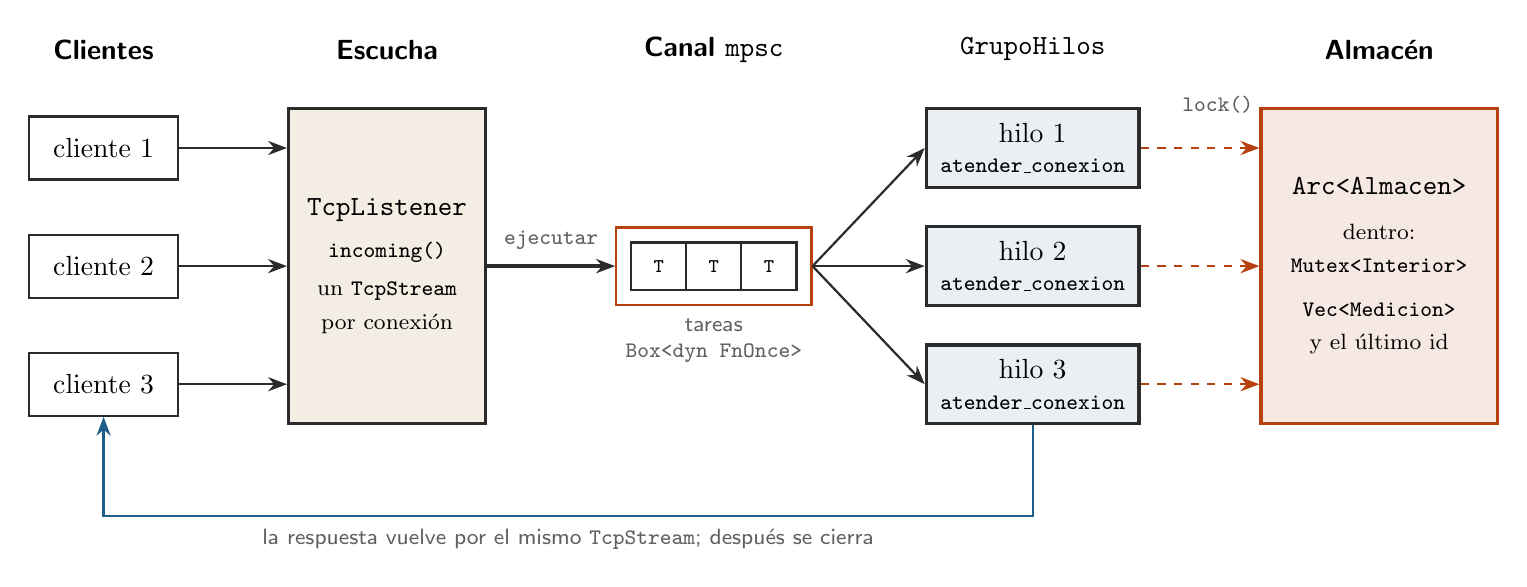
\begin{tikzpicture}[>={Stealth[length=2.4mm]},
  execute at begin node={\hyphenpenalty=10000},
  caja/.style={draw=carbon,very thick,fill=arena,align=center,
    minimum height=9mm,inner sep=4pt},
  cli/.style={draw=carbon,thick,fill=white,minimum width=19mm,
    minimum height=8mm,align=center},
  hilo/.style={draw=carbon,very thick,fill=azul!10,minimum width=27mm,
    minimum height=10mm,align=center},
  tarea/.style={draw=carbon,thick,fill=white,minimum width=7mm,
    minimum height=6mm,font=\ttfamily\scriptsize},
  rotulo/.style={font=\sffamily\footnotesize,text=carbon!75},
  titulo/.style={font=\sffamily\bfseries}]
  % Clientes
  \node[titulo] at (0,2.75) {Clientes};
  \foreach \i/\y in {1/1.5,2/0,3/-1.5} {\node[cli] (c\i) at (0,\y) {cliente \i};}
  % Escucha
  \node[titulo] at (3.6,2.75) {Escucha};
  \node[caja,minimum width=25mm,minimum height=40mm] (tl) at (3.6,0)
    {\texttt{TcpListener}\\[3pt]\footnotesize\texttt{incoming()}\\[2pt]
     \footnotesize un \texttt{TcpStream}\\\footnotesize por conexión};
  \foreach \i in {1,2,3} {\draw[->,thick,carbon] (c\i.east) -- (c\i.east -| tl.west);}
  % Canal con tareas
  \node[titulo] at (7.75,2.75) {Canal \texttt{mpsc}};
  \foreach \k in {0,1,2} {\node[tarea] (t\k) at (7.05+\k*0.7,0) {T};}
  \node[draw=oxido,thick,inner sep=5pt,fit=(t0)(t2)] (cola) {};
  \node[rotulo,align=center] at (7.75,-0.95) {tareas\\\texttt{Box<dyn FnOnce>}};
  \draw[->,very thick,carbon] (tl.east) -- node[rotulo,above=2pt] {\texttt{ejecutar}} (cola.west);
  % Grupo de hilos
  \node[titulo] at (11.8,2.75) {\texttt{GrupoHilos}};
  \foreach \i/\y in {1/1.5,2/0,3/-1.5} {
    \node[hilo] (h\i) at (11.8,\y) {hilo \i\\[-1pt]\footnotesize\ttfamily atender\_conexion};}
  \foreach \i in {1,2,3} {\draw[->,thick,carbon] (cola.east) -- (h\i.west);}
  % Almacén
  \node[titulo] at (16.2,2.75) {Almacén};
  \node[caja,fill=oxido!12,draw=oxido,minimum width=30mm,minimum height=40mm] (al) at (16.2,0)
    {\texttt{Arc<Almacen>}\\[4pt]\footnotesize dentro:\\\footnotesize\texttt{Mutex<Interior>}\\[4pt]
     \footnotesize\texttt{Vec<Medicion>}\\\footnotesize y el último id};
  \foreach \i in {1,2,3} {\draw[->,thick,oxido,dashed] (h\i.east) -- (h\i.east -| al.west);}
  \node[rotulo] at (14.15,2.05) {\texttt{lock()}};
  % Respuesta
  \draw[->,thick,azul] (h3.south) -- ++(0,-1.15) -| node[rotulo,pos=0.25,below=1pt]
    {la respuesta vuelve por el mismo \texttt{TcpStream}; después se cierra} (c3.south);
\end{tikzpicture}
\end{document}
